% !TEX root =  ../main_manuscript.tex 

\section{Introduction}
\label{sec:introduction}
Prostate cancer is the second most frequently diagnosed cancer in men worldwide \cite{GlobalCancerStats2012}. In prostate cancer screening programs, many of the diagnosed tumors are clinically insignificant (over-diagnosed) \cite{etzioni2002overdiagnosis}. To avoid further over-treatment, patients diagnosed with low-grade prostate cancer are commonly advised to join active surveillance (AS) programs. In AS, invasive treatments such as surgery are delayed until cancer progresses. Cancer progression is routinely monitored via serum prostate-specific antigen (PSA) measurements, a protein biomarker; digital rectal examination (DRE) measurements, a measure of the size and location of the tumor; and biopsies.

While larger values for PSA and/or DRE, may indicate cancer progression, biopsies are the most reliable cancer progression examination technique used in AS. When a patient's biopsy Gleason score becomes larger than 6 (positive biopsy, cancer progression detected), AS is stopped and the patient is advised treatment \cite{bokhorst2015compliance}. However, biopsies are invasive, painful, and prone to medical complications \cite{ehdaie2014impact,fujita2009serial}. Hence, they are conducted intermittently until a positive biopsy. Consequently, at the time of a positive biopsy, cancer progression may be observed with a delay of unknown duration. This delay is defined as the difference between the time of the positive biopsy and the unobserved true time of cancer progression. Thus, the decision to conduct biopsies requires a compromise between the burden of biopsy and the potential delay in the detection of cancer progression.

In AS, a delay in the detection of cancer progression around 12 to 14 months is assumed to be unlikely to substantially increase the risk of adverse downstream outcomes \cite{inoue2018comparative,carvalho}. However, for biopsies, there is little consensus on the time gap between them \cite{loeb2014heterogeneity,bruinsma2016active,nieboer2018active}. Many AS programs focus on minimizing the delay in the detection of cancer progression, by scheduling biopsies annually for all patients. A drawback of annual biopsies, and other currently practiced fixed/heuristic schedules \cite{loeb2014heterogeneity,bruinsma2016active,nieboer2018active}, is that they ignore the large variation in the time of cancer progression of AS patients. While they may work well for patients who progress early (\textit{fast progressing}) in AS, but for a large proportion of patients who do not progress, or progress late (\textit{slow progressing}) in AS, many unnecessary burdensome biopsies are scheduled. To mediate the burden between the \textit{fast} and \textit{slow progressing} patients, the world's largest AS program, Prostate Cancer Research International Active Surveillance\cite{bokhorst2016decade} (PRIAS), schedules annual biopsies only for patients with a low PSA doubling time \cite{bokhorst2015compliance}. For everyone else, PRIAS schedules biopsies at following fixed follow-up times: year one, four, seven, and ten, and every five years thereafter. Despite this effort in PRIAS, patients may get scheduled for four to ten biopsies over a period of ten years. Therefore, compliance for biopsies is low in PRIAS \cite{bokhorst2015compliance}. This can lead to a delay in the detection of cancer progression, and reduce the effectiveness of AS.

%Five reasons for why median and not mean:
%1. mean has decimals, hard to interpret
%2. median and IQR are useful coz distributions are skewed
%3. median also corresponds to 50% of those patients who never progress. Thus X axis is also having the interpretation: Burden for patients who never progress. and Y-axis: median benefit for patients who progress at the burden of those who never progress.
%4. no point showing mean for this plot and showing median (IQR) everywhere else
%5. decision making is easier for % of patients, e.g. median is 50% patients, and Q3 is 75% patients

We aim to better balance the number of biopsies (more are burdensome), and the delay in the detection of cancer progression (less is beneficial), than currently practiced schedules. We intend to achieve this by personalizing the decision to conduct biopsies (see Figure~\ref{fig:obsDataPlot_2340}). These decisions are made at a patient's pre-scheduled follow-up visits for DRE and PSA measurements. To develop the personalized decision making methodology, we utilize the data of the patients enrolled in the PRIAS study. We model this data and develop the personalized approach using joint models for time-to-event and longitudinal data \cite{tsiatis2004joint,rizopoulos2012joint}. In order to compare the personalized approach with current schedules, we conduct an extensive simulation study based on a replica of the patients from the PRIAS program. 

%\begin{figure}[!htb]
%\captionsetup{justification=justified}
%\centerline{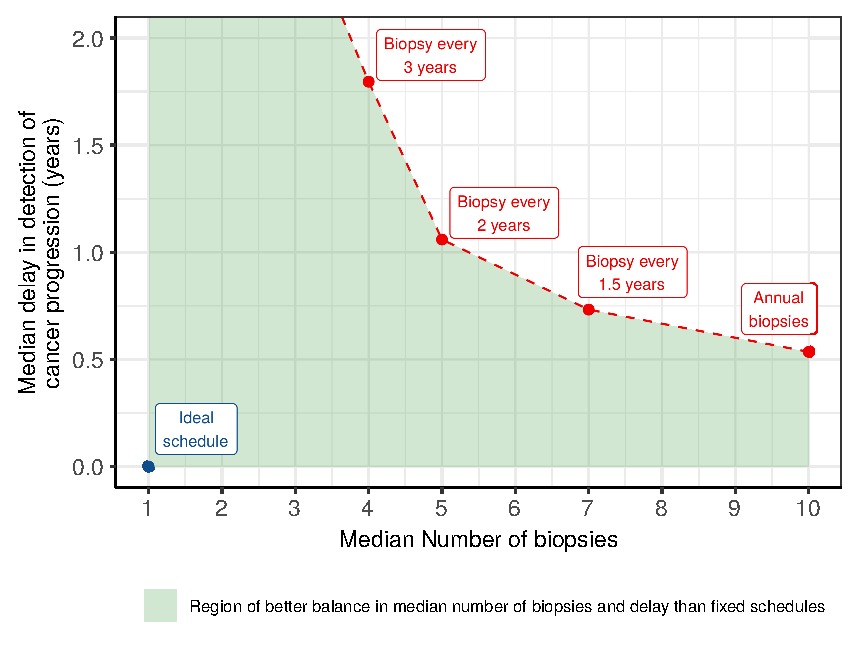
\includegraphics[width=\columnwidth]{images/better_balance_intro.eps}}
%\caption{\textbf{Burden-benefit frontier:} Estimated median number of biopsies, and median delay in the detection of cancer progression, due to various currently practiced fixed/heuristic biopsy schedules (red squares), over a follow-up of ten years. These are based on cancer progression times simulated using inversion sampling from the cumulative risk of cancer progression observed in PRIAS study (see Figure~\ref{fig:npmle_plot} and \hyperref[subsec:study_population]{Study Population} section). Using personalized decision making for biopsies, we intend to better balance the number of biopsies and the delay (green region), than currently practiced schedules. An ideal biopsy schedule (blue circle) will schedule only one biopsy, exactly at the true time of cancer progression.}
%\label{fig:better_balance_intro}
%\end{figure}

\begin{figure}[!htb]
\captionsetup{justification=justified}
\centerline{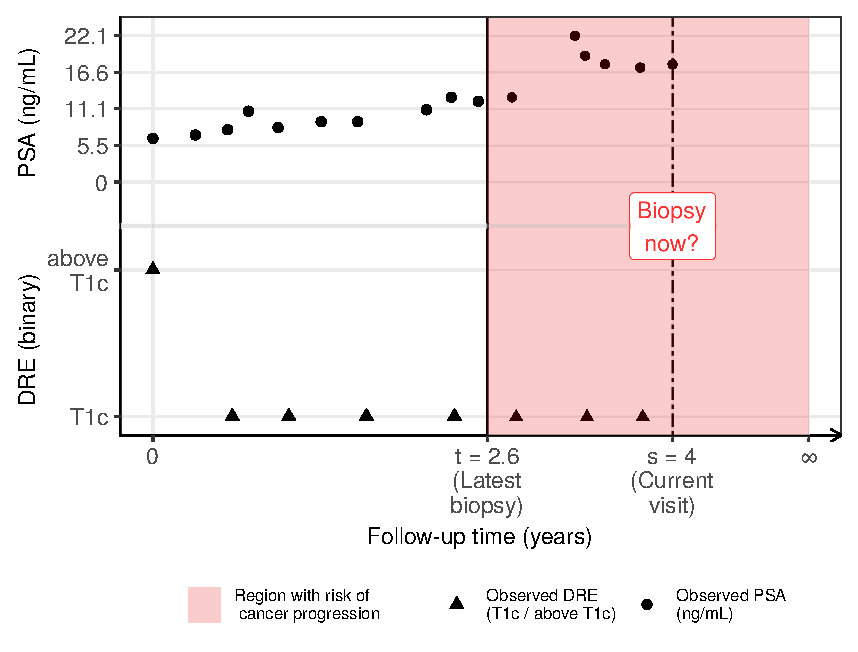
\includegraphics[width=\columnwidth]{images/obsDataPlot_2340.eps}}
\caption{\textbf{The personalized decision making problem:} Available data of a patient $j$, who had his latest negative biopsy at $t=2.6$ years. The shaded region shows the time period in which the patient is at risk of cancer progression. His current pre-scheduled follow-up visit for measurement of DRE and PSA is at $s=4$ years. Using his entire history of DRE $\mathcal{Y}_{dj}(s)$ and PSA $\mathcal{Y}_{pj}(s)$ measurements up to the current visit $s$, and the time of the latest biopsy $t$, we intend to make a decision on scheduling a biopsy at the current visit.}
\label{fig:obsDataPlot_2340}
\end{figure}

%The rest of the article is structured as follows: The details of the joint modeling framework and the biopsy decision making methodology are presented in the \hyperref[sec:methods]{Methods} section. The details of the simulation study and the corresponding results are presented in \hyperref[sec:methods]{Methods} and \hyperref[sec:results]{Results} sections, respectively. We conclude the paper with a \hyperref[sec:discussion]{Discussion} section.